\documentclass{article}
\usepackage[utf8]{inputenc}
\usepackage{minted}
\usepackage{graphicx}
\setminted{fontsize=\footnotesize,baselinestretch=1}

\title{Shared Memory Code Generation with Thorin}
\author{Rafael Ravedutti Lucio Machado }
\date{November 2017}

\begin{document}

\maketitle

\clearpage

\tableofcontents

\clearpage

\section{Introduction}
AnyDSL is a framework designed for the development of domain specific libraries, it allows developers to split their work in application developer, DSL designer and machine expert by using higher-order functions to abstract the lower levels of code. In the end, all the parts of the program are linked to build the program for the specified hardware.

The approximation above has a drawback, higher-order functions requires a language that supports functions as parameters of other functions, this may lead to a considerable overhead in the final application. For this purpose, the Thorin graph-based intermediate representation is used to reduce any overhead that this approach may cause.

For this work, we write a simple Gaussian filter using the AnyDSL front-end language Impala, this version uses a machine code to run in CUDA GPUs, but no references for shared memory are written in the original Impala code, instead, we modify the Thorin backend code generator for CUDA so it can generate the shared memory parts in the final code.

This report shows the methods used for allowing Thorin code generator to emit the optimized version of the Gaussian Filter (and other simple filters) using the GPU shared memory (CUDA to be more precisely). The first part explains the methodology used for generating the shared memory code for both image and filter and the second shows the modifications included in the Thorin backend code generator.

\section{Methodology}
Thorin is a CPS graph based higher-order intermediate representation, this means that its code generator will iterate over the graph generating its continuations, parameters and primops. For each vertex in the graph, Thorin must generate a unique name to avoid conflicts, our idea is to trace some of these vertex by the name to identify the filters and images in the kernel parameters (we also use the names of the structures in our experimental DSL in Impala for this).

After knowing the images and filters in the kernel, we trace their buffers so we know if they are read-only buffers or if at some point in the code they will be written. In the second case, we ignore them as we don't want to store writable buffers in the shared memory.

In the first step of the code generation we define a macro with the filter size used, then at each kernel declaration, we get the kernel block dimensions and emit the shared memory buffer declarations for both image and filter.

Before the next code generation we go through the Thorin graph to perform an initial analysis, going through the kernel primops to check the parameters behavior, if an extraction, a bitcast or a LEA operation is performed on a buffer that comes from an image or filter of the kernel, we keep saving the sources. This step are used for the read-only buffers tracing technique mentioned above. When we find a load operation in one of our targets, we insert them in the shared memory candidates list if they weren't blacklisted yet. A target is blacklisted when a store operation is performed in it (we don't want to store writable kernel buffers in the shared memory).

After the analysis, we go generating the code and for each bitcasting operation with the targets we emit the shared memory copy of the original buffer in the slow global memory to the faster memory by splitting the buffer in blocks of the kernel block dimension. Then we iterate over each buffer blocks with each thread transferring one element (per iteration) from the global memory to the faster memory. Finally, for each LEA operation with a target, we change the target reference to the shared memory with the offsets (x and y axis) included in the indexes.

This methodology of listing the candidates, tracing their path to know which ones are read-only and then during the code generation generating the copy and replacing the accesses for the candidates is used on this work to perform the shared memory code generation. The next section shows the code changed in the Thorin code generator for a practical guide through this work's idea.

\section{Modifications}

We use lists (C++ \textbf{std::list}) to perform the analysis, the \textbf{kernel\_images} and \textbf{kernel\_filters} lists will contain all the image and filter references from the kernel, respectively. The \textbf{image\_pointers} and \textbf{filter\_pointers} lists will have all the direct and indirect references to the image and filter buffers, respectively (doesn't matter which type these references have). The \textbf{shm\_buffers} list will contain all the selected buffers that must go to the shared memory and the \textbf{shm\_blacklist} will contain all the blacklisted buffers. The \textbf{std::map} object \textbf{conv\_map} contains the association between \textbf{image\_pointers} and \textbf{filter\_pointers} objects and their \textbf{shm\_buffers} object.

\subsection{Data structures}

\begin{minted}{cpp}
static std::list<std::string> shm_buffers;
static std::list<std::string> shm_blacklist;
static std::list<std::string> kernel_images;
static std::list<std::string> kernel_filters;
static std::list<std::string> image_pointers;
static std::list<std::string> filter_pointers;
static std::map<std::string, std::string> conv_map;
\end{minted}

The following code shows the functions that emits the copy from the global memory to the shared memory for an image giving the shared memory name \textbf{shm\_name} and the source buffer pointer \textbf{src\_buffer} name to be copied. The \textbf{adjusted\_(shm\_name)} definition in the end of the code is used for further accesses into the shared memory. \textbf{FILTER\_SIZE} holds the filter size.

\pagebreak

\subsection{Image shared memory functions}

\begin{minted}{cpp}
std::ostream& CCodeGen::emit_shm_image_copy(const std::string shm_name, const std::string src_buffer) {
  int extend_width = FILTER_SIZE / 2;
  int extend_height = FILTER_SIZE / 2;

  std::string idxx_string = "gidx - " + std::to_string(extend_width) + " + i";
  std::string idxy_string = "gidy - " + std::to_string(extend_height) + " + j";

  func_impl_ << endl;

  func_impl_ << "#line 100 \"shared_memory_image_copy\"" << endl;
  func_impl_ << "int gidx = blockIdx.x * blockDim.x + threadIdx.x;" << endl;
  func_impl_ << "int gidy = blockIdx.y * blockDim.y + threadIdx.y;" << endl;

  func_impl_ << "for(int i = 0; threadIdx.x + i < blockDim.x + " << extend_width * 2 << "; i += blockDim.x) {" << up << endl;
  func_impl_ << "int idxx = " << idxx_string << ";" << endl;

  func_impl_ << "for(int j = 0; threadIdx.y + j < blockDim.y + " << extend_height * 2 << "; j += blockDim.y) {" << up << endl;
  func_impl_ << "int idxy = " << idxy_string << ";" << endl;

  func_impl_ << "if(idxx < image_width_reg && idxy < image_height_reg) {" << up << endl;

  func_impl_ << shm_name << "[(threadIdx.y + j) * " << shm_width << " + threadIdx.x + i] = " << \
                src_buffer << "[idxy * image_width_reg + idxx];" << down << endl;

  func_impl_ << "}" << down << endl;
  func_impl_ << "}" << down << endl;
  func_impl_ << "}" << endl;

  func_impl_ << endl << "__syncthreads();" << endl;

  func_impl_ << endl << "double *adjusted_" << shm_name << " = &" << shm_name << \
                        "[(" << extend_height << " - blockIdx.y * blockDim.y) * " << shm_width << \
                        " + " << extend_width << " - blockIdx.x * blockDim.x];" << endl;

  return func_impl_;
}
\end{minted}

The following code shows the function that emits the shared memory access for an image giving its name in \textbf{shm\_name} and its \textbf{x} and \textbf{y} positions.

\begin{minted}{cpp}
std::ostream& CCodeGen::emit_shm_image_access(const std::string shm_name, std::string x, std::string y) {
  func_impl_ << "&" << "adjusted_" << shm_name << "[(" << y  << ") * " << shm_width << " + (" << x << ")]";

  return func_impl_;
}
\end{minted}

\subsection{Filter shared memory functions}

The following code shows the functions that emits the copy from the global memory to the shared memory for a filter giving the shared memory name \textbf{shm\_name} and the source buffer pointer \textbf{src\_buffer} name to be copied. The \textbf{SEP\_FILTER} macro defines if it's an unidimensional separable filter or it's a bidimensional block filter. \textbf{FILTER\_SIZE} contains the filter size.

\pagebreak

\begin{minted}{cpp}
std::ostream& CCodeGen::emit_shm_filter_copy(const std::string shm_name, const std::string src_buffer) {
  std::string idx_string;

  func_impl_ << endl;

  func_impl_ << "#line 200 \"shared_memory_filter_copy\"" << endl;

#ifdef SEP_FILTER
  idx_string = "i";

  func_impl_ << "for(int i = 0; i < " << FILTER_SIZE << "; i++) {" << up << endl;
  func_impl_ << shm_name << "[" << idx_string << "] = " << src_buffer << "[" << idx_string << "];" << down << endl;

  func_impl_ << "}" << endl;
#else
  idx_string = "(threadIdx.y + j) * " + std::to_string(FILTER_SIZE) + " + threadIdx.x + i";

  func_impl_ << "for(int i = 0; i < " << FILTER_SIZE << "; i += blockDim.x) {" << up << endl;
  func_impl_ << "for(int j = 0; j < " << FILTER_SIZE << "; j += blockDim.y) {" << up << endl;
  func_impl_ << "if(threadIdx.x + i < " << FILTER_SIZE << " && " << endl << \
                "   threadIdx.y + j < " << FILTER_SIZE << ") {" << up << endl;

  func_impl_ << shm_name << "[" << idx_string << "] = \\" << endl << \
                "  " << src_buffer << "[" << idx_string << "];" << down << endl;

  func_impl_ << "}" << down << endl;
  func_impl_ << "}" << down << endl;
  func_impl_ << "}" << endl;
#endif

  func_impl_ << endl << "__syncthreads();" << endl;

  return func_impl_;
}
\end{minted}

The following code shows the function that emits the shared memory access for a filter giving its name in \textbf{shm\_name} and the index \textbf{index} to be accessed.

\begin{minted}{cpp}
std::ostream& CCodeGen::emit_shm_filter_access(const std::string shm_name, std::string index) {
  func_impl_ << "&" << shm_name << "[" << index << "]";

  return func_impl_;
}
\end{minted}

\subsection{Kernel image and filter identification}

The following code will use our experimental DSL structure names \textbf{image} and \textbf{filter} to select the kernel parameters that are images or filters. We also include the AnyDSL structure \textbf{Buffer} to be considered as images because of the second kernel in the separable convolution that receives the image as \textbf{Buffer} instead of \textbf{image}.

\begin{minted}{cpp}
std::stringstream type_stream;

type_stream << param->type();

if(type_stream.str().compare("filter") == 0 && !list_contains(kernel_filters, param->unique_name())) {
  kernel_filters.push_back(param->unique_name());
}

if(type_stream.str().compare("image") == 0 && !list_contains(kernel_images, param->unique_name())) {
  image_width_name = param->unique_name() + ".e2";
  image_height_name = param->unique_name() + ".e3";
  kernel_images.push_back(param->unique_name());
}

if(type_stream.str().compare("Buffer") == 0 && !list_contains(kernel_images, param->unique_name())) {
  kernel_images.push_back(param->unique_name());
}
\end{minted}

The \textbf{e2} and \textbf{e3} elements in the image strucuture holds the image width and height, respectively.

\subsection{Shared memory declarations}

The following code emits the shared memory declaration in the kernel using the \textbf{FILTER\_SIZE} macro.

\begin{minted}{cpp}
if(bdimx != 0 && bdimy != 0 && bdimz != 0) {
  shm_width = bdimx + (FILTER_SIZE / 2) * 2;
  func_impl_ << endl << "__shared__ double ds_img[" << (shm_width * (bdimy + (FILTER_SIZE / 2) * 2)) << "];";

  #ifdef SEP_FILTER
    func_impl_ << endl << "__shared__ double ds_filter[" << FILTER_SIZE << "];";
  #else
    func_impl_ << endl << "__shared__ double ds_filter[" << (FILTER_SIZE * FILTER_SIZE) << "];";
  #endif
}
\end{minted}

\subsection{Read-only buffers tracing}

The following code is executed before the code generation, it perform our analysis of possible candidates to be optimized using the shared memory.

\begin{minted}{cpp}
for(const auto& block : schedule) {
  auto continuation = block.continuation();
  if(continuation->empty()) {
    continue;
  }

  assert(continuation == scope.entry() || continuation->is_basicblock());

  for(auto primop : block) {
    auto primop_name = var_name(primop);

    if(auto aggop = primop->isa<AggOp>()) {
      if(aggop->isa<Extract>()) {
        if(list_contains(kernel_images, aggop->agg()->unique_name())) {
          if(aggop->type()->isa<StructType>() && !list_contains(kernel_images, primop_name)) {
            kernel_images.push_back(primop_name);
          } else if(aggop->type()->isa<PtrType>() && !list_contains(image_pointers, primop_name)) {
            image_pointers.push_back(primop_name);
          }
        }

        if(list_contains(kernel_filters, aggop->agg()->unique_name())) {
          if(aggop->type()->isa<StructType>() && !list_contains(kernel_filters, primop_name)) {
            kernel_filters.push_back(primop_name);
          } else if(aggop->type()->isa<PtrType>() && !list_contains(filter_pointers, primop_name)) {
            filter_pointers.push_back(primop_name);
          }
        }
      }
    } else if(auto conv = primop->isa<ConvOp>()) {
      if(conv->isa<Bitcast>()) {
        if(list_contains(image_pointers, conv->from()->unique_name())) {
          image_pointers.push_back(primop_name);
        }

        if(list_contains(filter_pointers, conv->from()->unique_name())) {
          filter_pointers.push_back(primop_name);
        }
      }
    } else if(auto lea = primop->isa<LEA>()) {
      if(list_contains(image_pointers, lea->ptr()->unique_name())) {
        conv_map.insert(std::pair<std::string, std::string>(lea->ptr()->unique_name(), primop_name));
        image_pointers.push_back(primop_name);
      }

      if(list_contains(filter_pointers, lea->ptr()->unique_name())) {
        conv_map.insert(std::pair<std::string, std::string>(lea->ptr()->unique_name(), primop_name));
        filter_pointers.push_back(primop_name);
      }
    } else if(auto load = primop->isa<Load>()) {
      auto ptr_name = load->ptr()->unique_name();
      auto blacklisted = list_contains(shm_blacklist, ptr_name);

      if(!blacklisted && (list_contains(image_pointers, ptr_name) || list_contains(filter_pointers, ptr_name))) {
        shm_buffers.push_back(ptr_name);
      }
    } else if(auto store = primop->isa<Store>()) {
      auto ptr_name = store->ptr()->unique_name();

      if(list_contains(shm_buffers, ptr_name)) {
        shm_buffers.remove(ptr_name);
      }

      shm_blacklist.push_back(ptr_name);
    }
  }
}
\end{minted}

\subsection{Dimension registers}

The next code generation is used to generate the registers \textbf{image\_width\_reg} and \textbf{image\_height\_reg} with the image dimensions. This is used so we have a known name for these values and also to avoid structure element access each time we use them.

\begin{minted}{cpp}
func_impl_ << endl;
func_impl_ << "int image_width_reg = " << image_width_name << ";" << endl;
func_impl_ << "int image_height_reg = " << image_height_name << ";" << endl;
\end{minted}

\subsection{Shared memory copy generation}

The code below shows the shared memory copy code generation after the bitcast operation (irrelevant parts of the code were omitted for legibility purposes).

\begin{minted}{cpp}
if (conv->isa<Bitcast>()) {
    ...

    if(list_contains(image_pointers, def_name)) {
      std::map<std::string, std::string>::iterator i;

      if((i = conv_map.find(def_name)) != conv_map.end()) {
        if(list_contains(shm_buffers, i->second)) {
          emit_shm_image_copy("ds_img", def_name);
        }
      }
    }

    if(list_contains(filter_pointers, def_name)) {
      std::map<std::string, std::string>::iterator i;

      if((i = conv_map.find(def_name)) != conv_map.end()) {
        if(list_contains(shm_buffers, i->second)) {
          emit_shm_filter_copy("ds_filter", def_name);
        }
      }
    }
}
\end{minted}

\subsection{Shared memory access generation}

Finally, the next code emits the shared memory access when necessary in the LEA operations (irrelevant parts of the code were omitted for legibility purposes).

\begin{minted}{cpp}
if (auto lea = def->isa<LEA>()) {
    if (is_texture_type(lea->type())) { // handle texture fetches
      ...
    } else {
        if (lea->ptr_pointee()->isa<TupleType>() || lea->ptr_pointee()->isa<StructType>()) {
          ...
        } else if (lea->ptr_pointee()->isa<DefiniteArrayType>()) {
          ...
        } else {
            if(list_contains(shm_buffers, def_name)) {
              func_impl_ << "#line 100 \"shared_memory_access\"" << endl;
            }

            emit_addr_space(func_impl_, lea->ptr()->type());
            emit_type(func_impl_, lea->type()) << " " << def_name << ";" << endl;
            func_impl_ << def_name << " = ";

            if(list_contains(shm_buffers, def_name)) {
                std::map<std::string, std::string>::iterator i;
                auto is_filter = list_contains(filter_pointers, def_name);

                if(!is_filter) {
                  emit_shm_image_access(
                    "ds_img",
                    lea->index()->unique_name() + " % image_width_reg",
                    lea->index()->unique_name() + " / image_width_reg"
                  );
                } else {
                  emit_shm_filter_access("ds_filter", lea->index()->unique_name());
                }

                func_impl_ << ";"; 
            } else { 
                emit(lea->ptr()) << " + ";
                emit(lea->index()) << ";"; 
            }
        }
    }

    ...
}
\end{minted}

\section{Experimental Results}

To perform the experiments and validate our generated code version performance, we use the Berkeley Segmentation Dataset [Martin et al., 2001] available at [Arbelaez et al., 2007], which contains 100 images with 321x481 and 481x321 dimensions. As these dimensions are too small for performance comparison, we use the same procedure as [Lourenço, 2011] to generate the variations with higher dimensions.

Considering the original dataset images as the B1 dataset, we generate the B2 dataset with the doubled dimensions by repeating the original images vertically, horizontally and diagonally. So, we repeat the same procedure on B2 to generate the B3 dataset, and the same on B3 to generate the B4 dataset. After all we have the following dimensions: 321x481 and 481x321 for B1 dataset, 642x962 and 962x642 for B2 dataset, 1284x1924 and 1924x1284 for B3 dataset and 2568x3848 and 3848x2568 for B4 dataset, all of them containing 100 images each.

The performance tests were performed using a GeForce GT 710B graphic board with 192 CUDA cores, 954MHz base clock, 2GB of memory with 1.8 Gbps of speed and a 64-bit DDR3 memory interface. We execute three different versions for all the images on each dataset and considered the summation of the times as the final result for our tests. The mentioned versions are named \textbf{no\_shm} for the original AnyDSL version that doesn't use shared memory, \textbf{shm\_filteronly} version that only uses shared memory for filter and \textbf{shm\_both} version that uses shared memory for both image and filter.

The Figure \ref{fig:results} shows the result in seconds for each dataset and the Table \ref{table:speedups} shows the speedups for \textbf{shm\_filteronly} and \textbf{shm\_both} versions.

\begin{figure}[!htb]
\centering
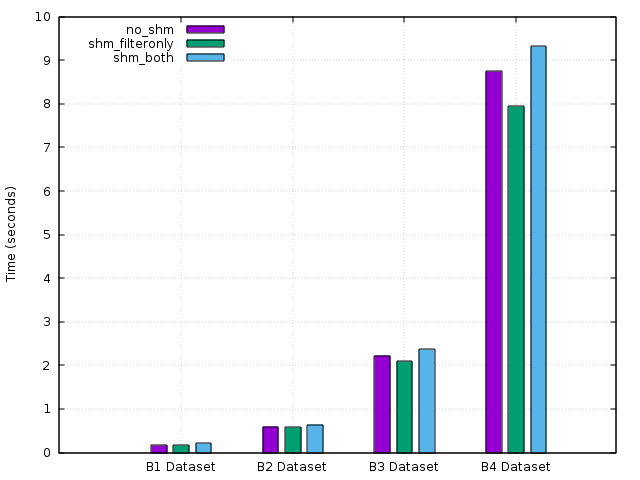
\includegraphics[width=13cm]{results.png}
\caption{Results for B1, B2, B3 and B4 datasets.}
\label{fig:results}
\end{figure}

\begin{table}
\centering
\begin{tabular}{ | c | c | c | c | c | }
  \hline
  & B1 & B2 & B3 & B4 \\
  \hline
  \textbf{shm\_filteronly} & 1.01144963524 & 1.01751663664 & 1.06079745639 & 1.10045501174 \\
  \hline
  \textbf{shm\_both} & 0.80856073526 & 0.92615324824 & 0.93869369236 & 0.93835056282 \\
  \hline
\end{tabular}
\caption{Speedups for \textbf{shm\_filteronly} and \textbf{shm\_both} versions}
\label{table:speedups}
\end{table}

The results shows that our version that only uses shared memory for filter is better than the original, while the version with both filter and image performed worse than the others. According to our analysis, this happened because of the emitted accesses for the image using the module and division functions with the image width to remap the original image index to the shared memory index.

\section{Future Work}
Future work may include a better way to remap the accesses from the global memory to the shared memory (by identifying the loops in the code and changing their range), as well as perform other kinds of optimizations during the code generation.

Another interesting work would be to perform the same optimizations for other GPU framework like OpenCL for example, then an analysis of performance using the modified version for a different architecture could be achieved.

\section{Conclusion}
The work in this report changes the Thorin generated code for the CUDA backends to include shared memory usage in the final version. We show better results for performance on inserting the filter into the shared memory and identified problems on remapping the image accesses to the shared memory (in relation to performance).

\section{References}

\end{document}

